\documentclass{article}
\usepackage[utf8]{inputenc}

\usepackage[utf8]{inputenc}
\usepackage[spanish,es-tabla,es-nodecimaldot]{babel}
\usepackage{amsmath,amsthm,amsfonts,amssymb,mathtools,dsfont,mathrsfs}
\usepackage{enumerate,graphicx,xcolor}
\usepackage{lmodern}
\usepackage[T1]{fontenc}
\usepackage[left=2cm,top=2.5cm,right=2cm,bottom=2.5cm]{geometry}
\usepackage[activate={true,nocompatibility},final,tracking=true,kerning=true,spacing=true,factor=1100,stretch=10,shrink=10]{microtype}
\usepackage{hyperref}


%\DeclarePairedDelimiter{\norm}{\lVert}{\rVert}




\newcommand{\N}{\mathbb{N}}
\newcommand{\R}{\mathbb R}
\newcommand{\Z}{\mathbb Z}
\newcommand{\Rbar}{\overline{\mathbb R}}
\newcommand{\F}{\mathscr F}
\newcommand{\A}{\mathscr A}
\newcommand{\To}{\Rightarrow}
\newcommand{\C}{\mathscr C}
\newcommand{\La}{\mathscr L_A}
\newcommand{\B}{\mathcal B}
\newcommand{\Q}{\mathbb Q}
\renewcommand{\epsilon}{\varepsilon}
\renewcommand{\L}{\mathcal L}
\renewcommand{\d}{\mathrm d}
\newcommand{\abs}[1]{\left| #1 \right|}
\newcommand{\pts}[1]{\left( #1 \right)}
\newcommand{\norm}[1]{\left\lVert#1\right\rVert}
\renewcommand{\P}[1]{\mathbb P\left( #1 \right)}
\newcommand{\E}[1]{\mathbb E \left( #1 \right)}


\newcommand{\ols}[1]{\mskip.5\thinmuskip\overline{\mskip-.5\thinmuskip {#1} \mskip-.5\thinmuskip}\mskip.5\thinmuskip} % overline short
\newcommand{\olsi}[1]{\,\overline{\!{#1}}} % overline short italic
\makeatletter
\newcommand\closure[1]{
  \tctestifnum{\count@stringtoks{#1}>1} %checks if number of chars in arg > 1 (including '\')
  {\ols{#1}} %if arg is longer than just one char, e.g. \mathbb{Q}, \mathbb{F},...
  {\olsi{#1}} %if arg is just one char, e.g. K, L,...
}
% FROM TOKCYCLE:
\long\def\count@stringtoks#1{\tc@earg\count@toks{\string#1}}
\long\def\count@toks#1{\the\numexpr-1\count@@toks#1.\tc@endcnt}
\long\def\count@@toks#1#2\tc@endcnt{+1\tc@ifempty{#2}{\relax}{\count@@toks#2\tc@endcnt}}
\def\tc@ifempty#1{\tc@testxifx{\expandafter\relax\detokenize{#1}\relax}}
\long\def\tc@earg#1#2{\expandafter#1\expandafter{#2}}
\long\def\tctestifnum#1{\tctestifcon{\ifnum#1\relax}}
\long\def\tctestifcon#1{#1\expandafter\tc@exfirst\else\expandafter\tc@exsecond\fi}
\long\def\tc@testxifx{\tc@earg\tctestifx}
\long\def\tctestifx#1{\tctestifcon{\ifx#1}}
\long\def\tc@exfirst#1#2{#1}
\long\def\tc@exsecond#1#2{#2}
\makeatother

\newtheorem{lemma}{Lema}
\newtheorem{theorem}{Teorema}

\setlength\parindent{0pt}
\setlength\parskip{4pt}


\title{Cómputo científico para probabilidad y estadística. Tarea 7.\\
MCMC: Metropolis-Hastings II}
\author{Juan Esaul González Rangel}
\date{Octubre 2023}



\begin{document}

\maketitle

\textbf{ \large Con el algoritmo Metropolis-Hastings (MH), simular lo siguiente: }

\begin{enumerate}

    \item Sean $x_i \sim Ga(\alpha, \beta); i = 1, 2, . . . , n$. Simular datos $x_i$ 
    con $\alpha = 3$ y $\beta = 100$ considerando los casos $n = 4$ y 30.
    
    Con $\alpha \sim U(1,4), \beta \sim exp(1)$ distribuciones a priori, se tiene la 
    posterior

    \[ f(\alpha, \beta | \bar x) \propto \frac{\beta^{n\alpha}}{\Gamma(\alpha)^n} 
    r_1^{\alpha - 1} e^{-\beta(r_2 + 1)} \mathds 1_{1 \le \alpha \le 4} 
    \mathds 1_{\beta > 0}, \]

    con $r_2 = \sum_{i=1}^n x_i$ y $r_1 = \prod_{i=1}^n x_i$.

    En ambos casos, grafica los contornos para visualizar dónde está concentrada la posterior.
    
    Utilizar la propuesta

    \[ q \left( \binom{\alpha_p}{\beta_p} \left| \binom{\alpha}\beta \right. \right) = 
    \binom{\alpha}{\beta} + \binom{\epsilon_1}{\epsilon_2}, \]

    donde

    \[ \binom{\epsilon_1}{\epsilon_2} \sim \mathcal N_2\left( \binom 00, \begin{pmatrix}
        \sigma_1^2 & 0 \\
        0 & \sigma_2^2
    \end{pmatrix} \right). \]



    \begin{proof}[Solución]

    La simulación de los datos Gamma($\alpha,\beta$) se realizó mediante Numpy, y se obtuvieron
    los siguientes valores,

    \begin{lstlisting}[language=Python]
data4 = [0.02458333 0.02352249 0.0602106  0.08239561]

data30 = [0.00271467 0.04123339 0.06655271 0.00750071 0.01409199 0.02545264
0.01677018 0.02412853 0.02313011 0.02021658 0.07463565 0.01992959
0.03853146 0.04940094 0.02968845 0.00975932 0.05164652 0.04375947
0.03710245 0.01255773 0.03329843 0.02368755 0.04556456 0.01107533
0.03635922 0.02969227 0.07078983 0.02011851 0.0694928  0.05073943]\end{lstlisting}

        A continuación, graficamos los contornos 

        \begin{center}
            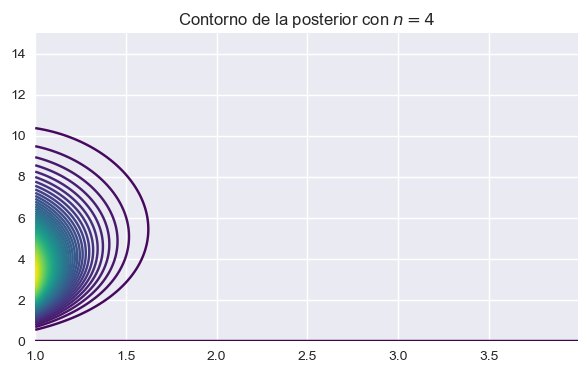
\includegraphics[width=0.6\textwidth]{tarea7/cont4.png}
            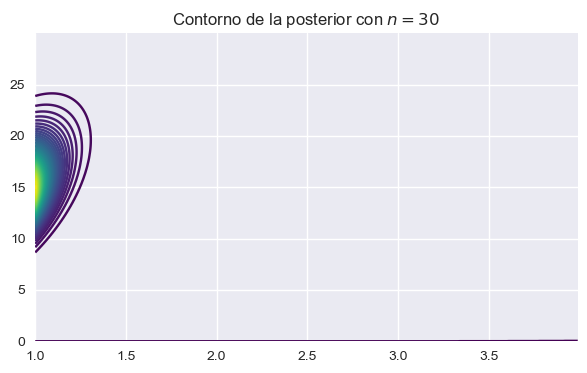
\includegraphics[width=0.6\textwidth]{tarea7/cont30.png}
        \end{center}

        Notamos que la densidad de la posterior parece estar concentrada en $0 \le \beta \le 10$ y
        $0 \le \alpha \le 1.75$ para el caso $n=4$, y en $7.5 \le \beta \le 25$ y $0\le \alpha \le 1.5$
        para $n=30$.

        Para muestrear de la posterior se implementó el algoritmo de Metropolis-Hastings usando la
        densidad de transición propuesta. Como distribución inicial se usó la constante con 
        $\alpha = 3, \beta=100$ con el objetivo de poder observar la evolución de la cadena desde
        un punto distante. La trayectoria de la cadena se muestra en la siguiente Figura.

        \begin{center}
            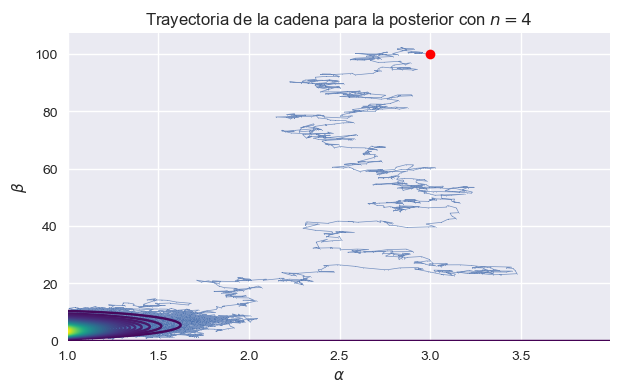
\includegraphics[width=0.7\textwidth]{tarea7/gamma4_norm.png}
        \end{center}

        El punto que se muestra en color rojo es el punto inicial de la cadena. 
        
        Podemos notar varias cosas, la primera es que en etapas tempranas de la cadena el
        movimiento es principalmente en sentido vertical, y esto es porque proporcionalmente,
        la componente $\alpha$ de la cadena se encuentra más cerca de la densidad que la componente
        $\beta$, lo que cause que se acepten las transiciones que hacen a $\beta$ más próximo,
        aunque no necesariamente lo hagan para $\alpha$. Eventualmente, la cadena parece moverse 
        con la misma intensidad en las direcciones $\alpha$ y $\beta$. 

        Para poder llegar a un comportamiento óptimo de la cadena, se ajustaron las varianzas
        $\sigma_1^2$ y $\sigma_2^2$, de manera que la cadena avanzara lo suficientemente rápido
        para llegar a la densidad en un tiempo corto, pero lo suficientemente lento, como para 
        permanecer en el dominio de concentración de la densidad una vez que se llegó ahí. Las
        desviaciones estándar que se usaron después de varios intentos son 0.05 y 0.5.

        Evidentemente, en esta cadena hay puntos que no corresponden a muestrear desde la 
        propuesta, por lo que es necesario encontrar el \textit{burn-in} y eliminar los primeros
        datos para contar con una muestra más fiel. Podemos estimar el momento en que la cadena 
        se estabiliza al observar la siguiente gráfica de $\log(f(\alpha_n,\beta_n))$, donde
        $f$ es la posterior.

        \begin{center}
            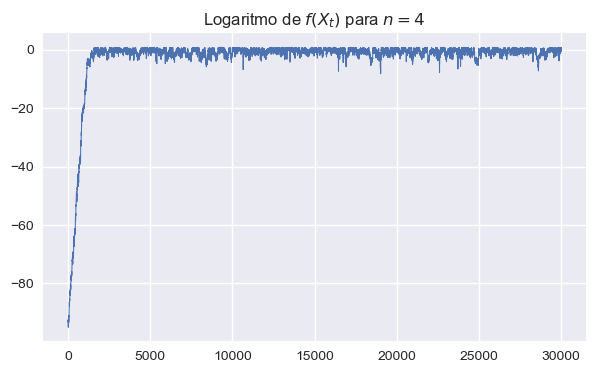
\includegraphics[width=0.7\textwidth]{tarea7/logdensgamma4.png}
        \end{center}

        Existe un punto en la evolución del proceso en el que el logaritmo de la densidad se estabiliza
        y podemos considerar que este es el momento a partir del cuál estamos muestreando desde 
        nuestra distribución objetivo. Entonces, para obtener una muestra de la posterior con la
        cadena, nos quedamos únicamente con las observaciones después de la 2,500. El histograma
        de dichas observaciones para $\alpha$ es el siguiente,

        \begin{center}
            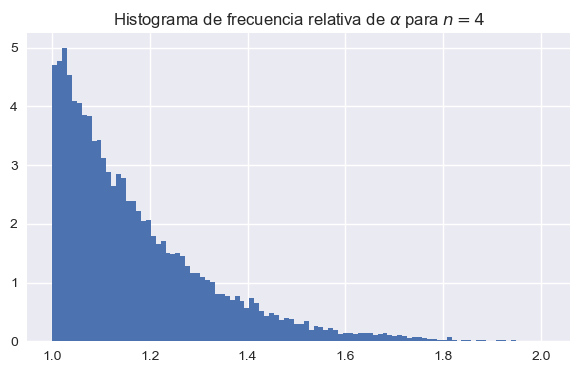
\includegraphics[width=0.7\textwidth]{tarea7/histalpha4.png}
        \end{center}

        El histograma correspondiente para $\beta$ es

        \begin{center}
            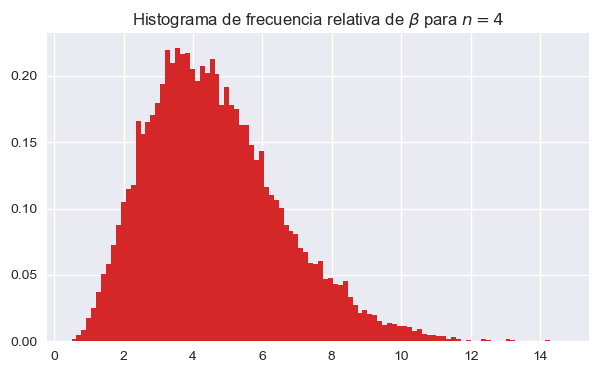
\includegraphics[width=0.7\textwidth]{tarea7/histbeta4.png}
        \end{center}

        Para el caso $n=30$ se tienen resultados simiares, la trayectoria de la cadena es la
        siguiente

        \begin{center}
            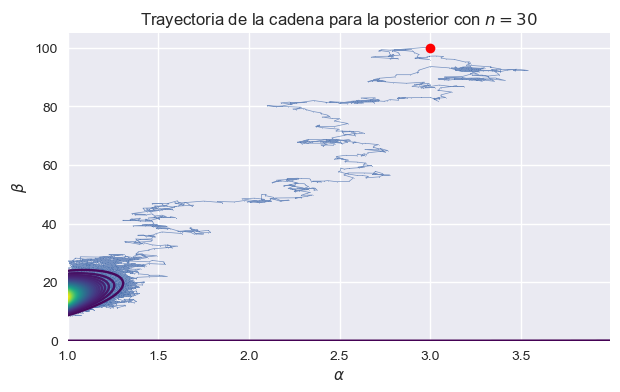
\includegraphics[width=0.7\textwidth]{tarea7/gamma30_norm.png}
        \end{center}

        De igual manera, el punto rojo es el punto inicial de la cadena. Notemos que en este caso
        la cadena se mueve en dirección a la densidad más rápidamente que en el anterior, y esto
        se puede deber a que ahora la densidad está más cerca del punto inicial, lo que causa que
        se rechace la transición con menos frecuencia.

        La gráfica de la log-densidad evaluada en la trayectoria es la siguiente,

        \begin{center}
            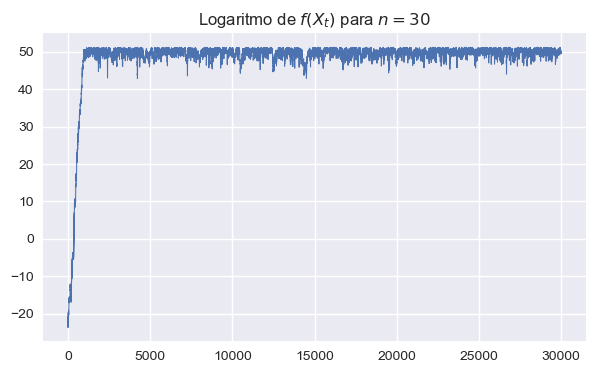
\includegraphics[width=0.7\textwidth]{tarea7/logdensgamma30.png}
        \end{center}

        En este caso, la log-densidad parece estabilizarse antes, por lo que es posible muestrear
        desde el punto 1500 en adelante. Al quedarnos únicamente con los valores pertinentes
        encontramos el siguiente histograma para $\alpha$

        \begin{center}
            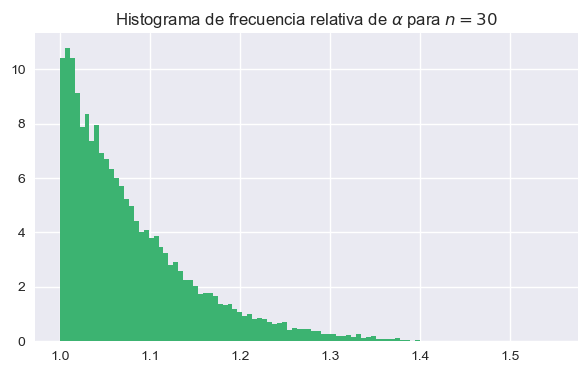
\includegraphics[width=0.7\textwidth]{tarea7/histalpha30.png}
        \end{center}

        El histograma correspondiente para $\beta$ es

        \begin{center}
            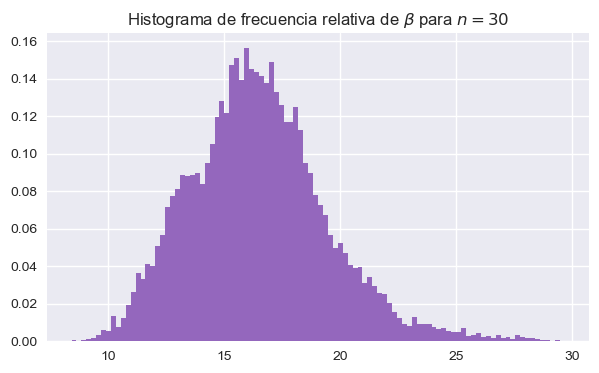
\includegraphics[width=0.7\textwidth]{tarea7/histbeta30.png}
        \end{center}

        En ambos casos, los resultados son similares a los que se obtienen para $n=4$.

        De un total de 30,000 pasos de la cadena que simulamos, se utilizaron alrededor de
        2,500 o 1,500 para comenzar a muestrear de la distribución objetivo. Teniendo en cuenta
        que el costo computacional de 2,500 pasos es relativamente bajo, tenemos que la cadena 
        es eficiente para la simulación de la posterior, pero debemos tener en cuenta que esto 
        se debe a que las varianzas fueron ajustadas para que la convergencia pueda ser los mejor
        posible. Así mismo, es posible ajustar aún más las varianzas o cambiar la distribución
        inicial para obtener una convergencia aún mejor a la distribución objetivo.

        Una alternativa a la distribución normal como transición es la distribución semicircular
        de Wigner. Al implementar el algoritmo de Metropolis-Hastings para el mismo problema con
        una semicircular obtenemos la siguiente trayectoria para $n=4$,

        \begin{center}
            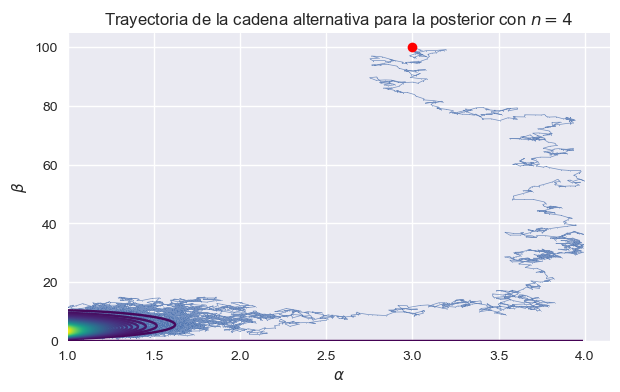
\includegraphics[width=0.7\textwidth]{tarea7/trajsemi4.png}
        \end{center}

        El comportamiento que observamos es similar al de la cadena con transición normal.
        Podemos encontrar su tasa de \textit{burn-in} usando la gráfica de log-densidad,

        \begin{center}
            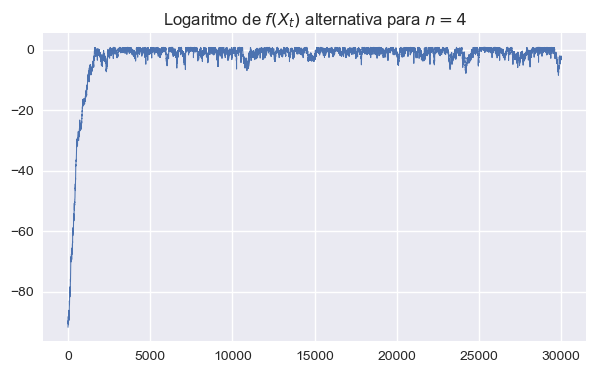
\includegraphics[width=0.7\textwidth]{tarea7/logsemic4.png}
        \end{center}

        Al igual que en el caso con densidad de transición normal, podemos considerar que
        es seguro tomar la muestra a partir del punto 2,500.

        Los histogramas que obtenemos para $\alpha$ y $\beta$ al eliminar los puntos de \textit{burn-in}
        son los siguientes,

        \begin{center}
            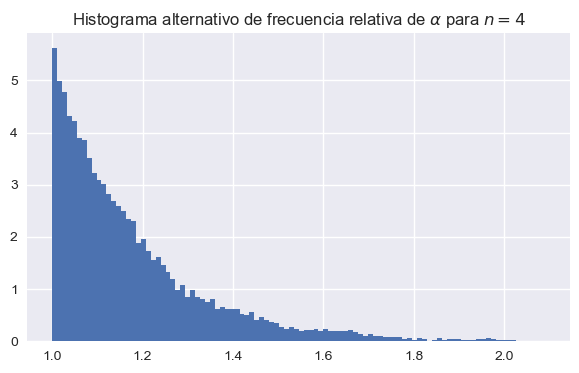
\includegraphics[width=0.6\textwidth]{tarea7/histalphasemic4.png}
            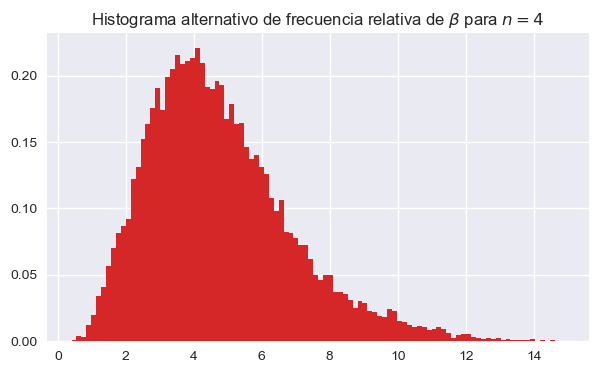
\includegraphics[width=0.6\textwidth]{tarea7/histbetasemic4.png}
        \end{center}

        Los resultados son similares al algoritmo con transición normal.

        Para el caso $n=30$ tenemos la siguiente trayectoria,

        \begin{center}
            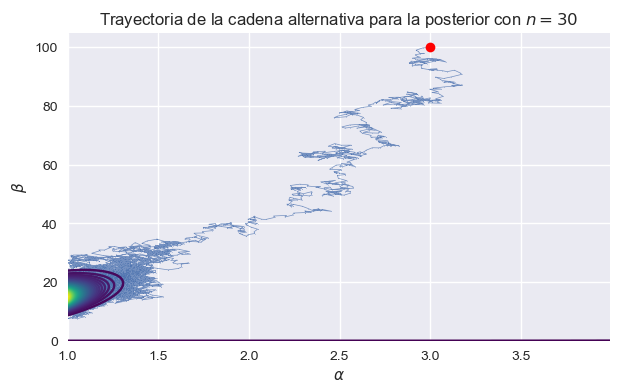
\includegraphics[width=0.63\textwidth]{tarea7/trajsemi30.png}
        \end{center}

        Al igual que en el caso de kernel normal, la cadena parece converger más rápido a la
        densidad que cuando $n=4$. En la siguiente figura se observa la log-densidad evaluada
        en la historia de la cadena,

        \begin{center}
            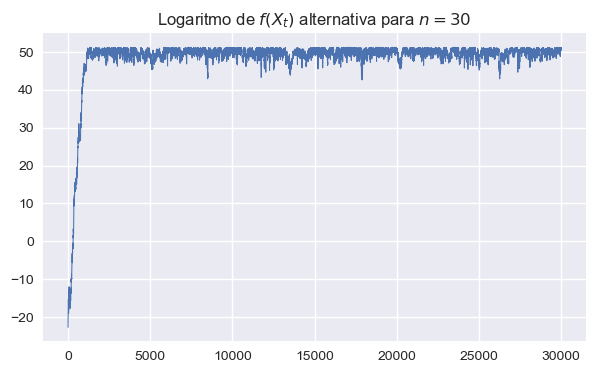
\includegraphics[width=0.65\textwidth]{tarea7/logsemic30.png}
        \end{center}

        Notamos que también en este caso es posible considerar el muestreo a partir de $1,500$
        iteraciones. Los histogramas para $\alpha$ y $\beta$ son los siguientes,

        \begin{center}
            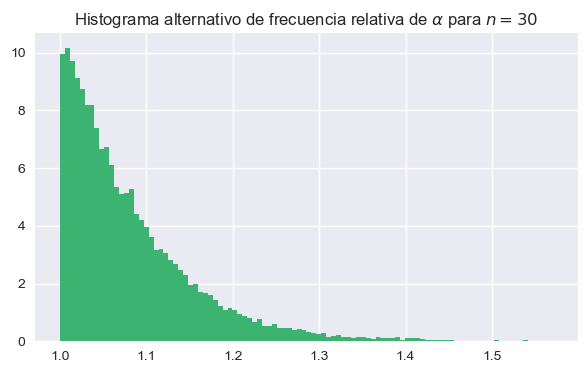
\includegraphics[width=0.65\textwidth]{tarea7/histalphasemic30.png}
            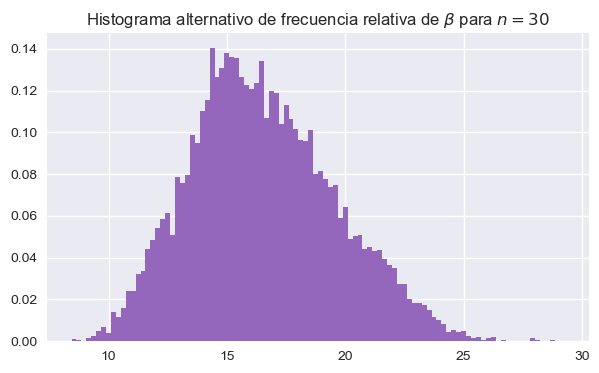
\includegraphics[width=0.65\textwidth]{tarea7/histbetasemic30.png}
        \end{center}

        Nuevamente, los resultados son similares a los análogos normales, por lo que concluimos
        que la distribución semicircular es una propuesta viable para este problema en 
        particular.



    \end{proof}



    \item Simular de la distribución Gamma$(\alpha,1)$ con la propuesta Gamma$([\alpha],1)$,
     donde $[\alpha]$ denota la parte entera de $\alpha$. 
    
    Además, realizar el siguiente experimento: poner como punto inicial $x_0 = 900$ y graficar
     la evolución de la cadena, es decir, $f (X_t)$ vs $t$.



    \begin{proof}[Solución]
        
        Primero debemos proponer un valor de $\alpha$. Es evidente que si $\alpha \in \Z$
        el problema no tiene sentido, pues en tal caso estaríamos usando simulaciones
        de $Ga(\alpha)$ para simular $Ga(\alpha)$, por lo que necesitamos que $\alpha$ no 
        sea entero, por ejemplo $\alpha = \pi$. Como lo dicta el ejercicio, establecemos el 
        punto inicial $x_0 = 900$, y obtenemos la siguiente trayectoria,

        \begin{center}
            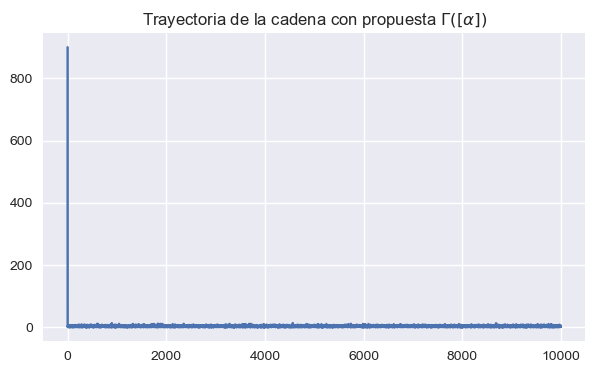
\includegraphics[width=0.75\textwidth]{tarea7/trajgamex2.png}
        \end{center}

        Como podemos notar, la cadena empieza en un punto muy alejado de la masa de la distribución,
        pero inmediantamente en un paso cambia a encontrarse dentro de él, y esto se debe a que,
        como la transición no depende del punto anterior, no importa dónde nos encontremos, siempre
        podemos llegar al soporte de la densidad en un paso (de hecho con probabilidad muy alta).

        La gráfica de $f(X_t)$ contra $t$, donde $f$ es la densidad objetivo, es la siguiente

        \begin{center}
            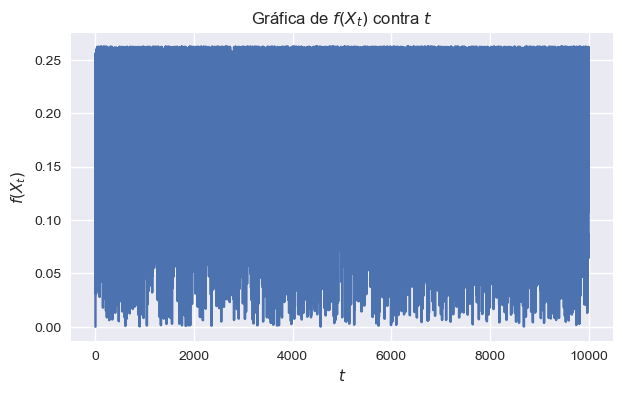
\includegraphics[width=0.65\textwidth]{tarea7/ft_t_traj.png}
        \end{center}

        Como sabemos que la densidad propuesta es muy cercana a la densidad objetivo, y la transición
        no depende del punto anterior, no es necesario realizar una gráfica de log-densidad para
        conocer el \textit{burn-in}, de hecho, es suficiente descartar el primer punto porque es
        el único que se encuentra fuera de las zonas donde la distribución objetivo concentra masa.
        Al descartar el primer punto obtenemos el siguiente histograma,

        \begin{center}
            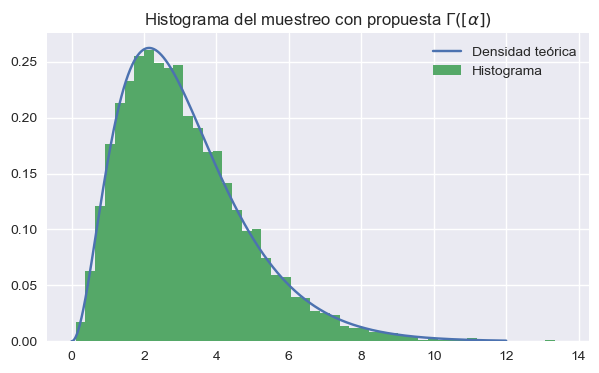
\includegraphics[width=0.65\textwidth]{tarea7/histgamex2.png}
        \end{center}
        
        El ajuste es bastante parecido a la densidad teórica. Esta cadena presenta una convergencia 
        muy rápida, y ella se debe a que contamos con una densidad de transición que es muy similar
        a nuestra densidad objetivo, lo que ocasiona que la transición se acepte con más frecuencia. 
        No siempre es posible contar con una densidad parecida a la densidad objetivo, por lo que 
        implementar una cadena como esta para muestrear desde cualquier distribución, en general
        no es posible.

        Observando el soporte de la distribución, nos damos cuenta de que la mayor parte de la masa se 
        concentra en el intervalo $(0,12)$, por lo que otra propuesta de transición razonable sería
        una uniforme en este intervalo. Al implementar el algoritmo con esta densidad de transición
        encontramos la siguiente trayectoria,

        \begin{center}
            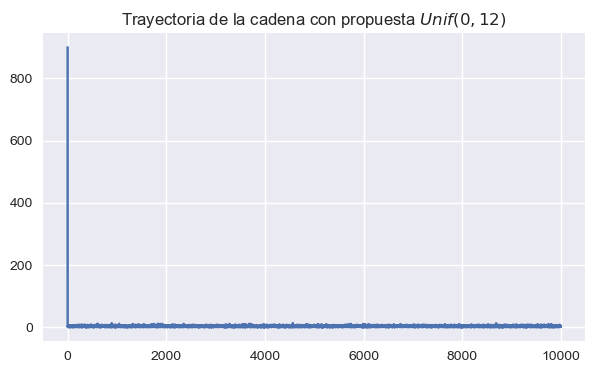
\includegraphics[width=0.65\textwidth]{tarea7/trajunifex2.png}
        \end{center}

        Como en el caso anterior, el hecho de que la propuesta no dependa del punto anterior, ocasiona
        que la trayectoria exhiba un comportamiento muy regular a partir del primer paso, pues se puede
        avanzar por todo el soporte de la densidad, importando únicamente la regla de rechazo de la
        transición. Similarmente, el \textit{burn-in} también consiste en quitar únicamente el
        primer punto, el histograma que obtenemos al hacer esto es,

        \begin{center}
            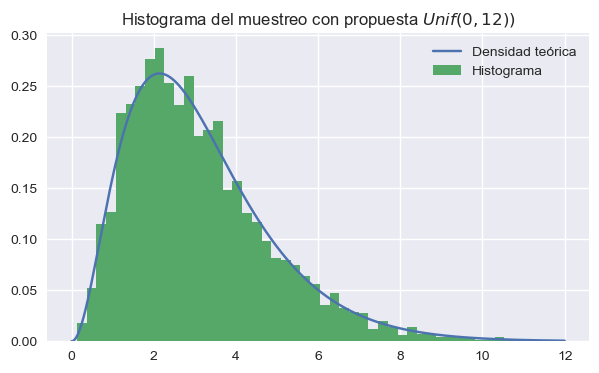
\includegraphics[width=0.65\textwidth]{tarea7/histunifex2.png}
        \end{center}

        El histograma ahora presenta un nivel de ajuste menor al de la cadena con propuesta $Ga([\alpha])$,
        ya que la distribución uniforme no es tan similar a la $Ga(\alpha)$. Aunque el diseño de la
        cadena garantiza la convergencia a la distribución objetvo, una mala elección de la densidad de
        transición puede ocasionar que esta convergencia sea más lenta. Podemos ver que cuando no tenemos
        una densidad de transición muy parecida a nuestra densidad objetivo, no es eficiente hacer
        una cadena cuya transición no dependa del punto anterior.
    \end{proof}



    \item Implementar Random Walk Metropolis Hasting (RWMH) donde la distribución objetivo 
    es $\mathcal N_2(\mu, \Sigma)$, con

    \[ \mu = \binom{3}{5} \quad \Sigma = \begin{pmatrix}
        1 & 0.9 \\
        0.9 & 1
    \end{pmatrix}. \]


    Utilizar como propuesta $\epsilon_t \sim \mathcal N_2 (\mathbf0, \sigma I)$. ¿Cómo elegir 
    $\sigma$ para que la cadena sea eficiente? ¿Qué consecuencias tiene la elección de $\sigma$?

    Como experimento, elige como punto inicial $x_o = \binom{1000}{1}$ y comenta los resultados.



    \begin{proof}[Solución]
        Al implementar el algoritmo con un $\sigma$ arbitrario, notamos que la longitud de los ``pasos''
        de la cadena está en función de $\sigma$. Un $\sigma$ muy chico ocasiona que la cadena se aleje
        muy poco del punto inicial, cubriendo una menor parte del soporte, o gastando demasiadas
        iteraciones en llegar a él. Un $\sigma$ grande permite que la cadena llegue más rápidamente a los
        puntos en que se concentra la masa de la distribución objetivo, pero también ocasiona
        que se tienda a abandonar esa zona con mucha frecuencia, lo que causa un muestreo más lento. Una
        elección de $\sigma$ adecuada permite que la cadena alcance la zona de muestreo de la distribución
        rápidamente y que permanezca en ella durante más tiempo.

        Mi elección de $\sigma$ se basó en probar con varios valores y observar el comportamiento 
        de la cadena al cubrir el plano, finalmente decidí utilizar $\sigma = 1/2$, pues con este
        valor se logra un equilibrio entre la velocidad con la que se muestrea, y la permanencia 
        en el soporte de la cadena.

        % 1000, 1

        Cuando intentamos iniciar la cadena en el punto $(1000,1)$ obtenemos un error de 
        división por 0, debido a que el punto $(1000,1)$ está lo suficientemente lejos de 
        la media de la densidad objetivo como para que la densidad evaluada en ese punto sea
        equivalente a cero en números de punto flotante. Con esto observamos que no cualquier
        punto dentro del dominio de la objetivo es una buena elección de punto inicial
        
        La trayectoria de la cadena con la densidad de transición propuesta y 
        punto inicial $(1,1)$ es la siguiente,

        \begin{center}
            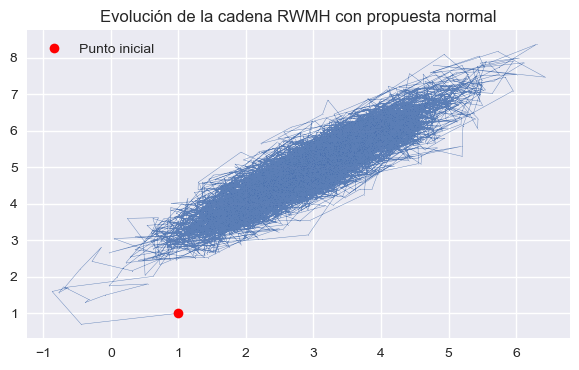
\includegraphics[width=0.7\textwidth]{tarea7/trajrwnorm.png}
        \end{center}

        Notemos que a pesar de comenzar en una zona fuera de la mayor concentración de masa de 
        la objetivo, la cadena rápidamente se concentra en una elipse alrededor de la media (3,5), y
        pasa la mayor parte de la trayectoria en esta zona. Se realizaron 10,000 iteraciones de esta
        cadena, pero debido a que llega muy rápido al dominio de la densidad objetivo, su función
        de log-densidad tiende a estabilizarse rápidamente, por lo que a continuación se muestra esta 
        función evaluada únicamente en los primeros 1,000 puntos,

        \begin{center}
            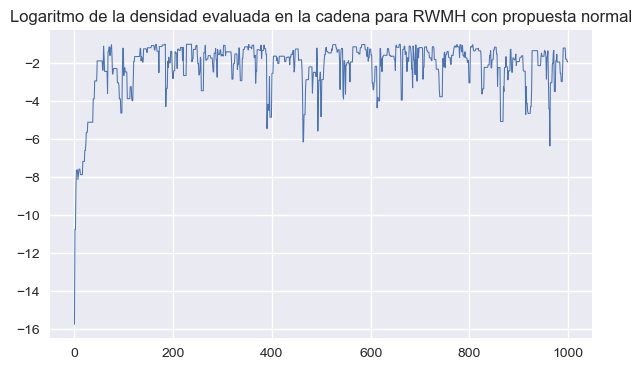
\includegraphics[width=0.7\textwidth]{tarea7/logdensrwnorm.png}
        \end{center}

        Podemos notar que es aproximadamente alrededor de la iteración 100 que la cadena comienza
        a encontrarse alrededor de la elipse que concentra la mayoría de la masa de la distribución.
        Los histogramas para ambas coordenadas al descartar en \textit{burn-in} son los siguientes,

        \begin{center}
            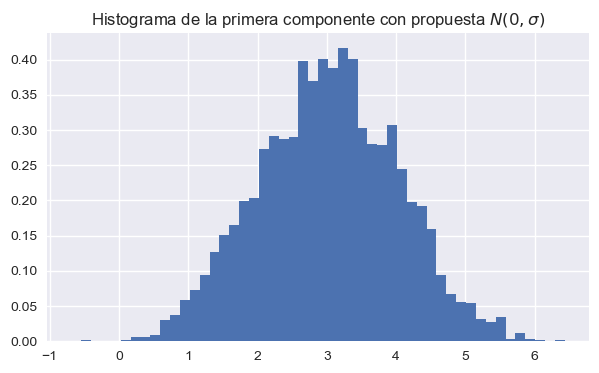
\includegraphics[width=0.7\textwidth]{tarea7/histrwnorm1.png}
            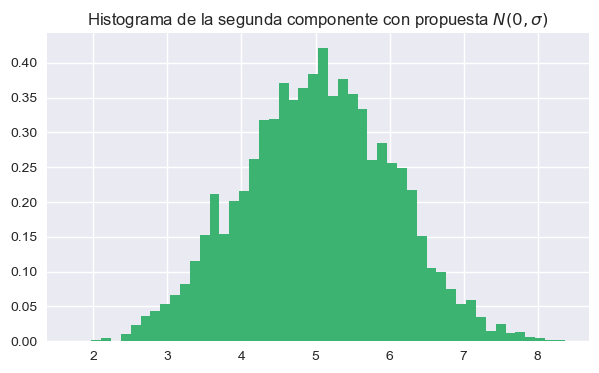
\includegraphics[width=0.7\textwidth]{tarea7/histrwnorm2.png}
        \end{center}

        Como se trata de un vector normal multivariado, sus marginales deben ser normales, aunque
        en este caso no son independientes.

        La velocidad de convergencia que observamos en las Figuras anteriores se debe tanto a la
        elección de la tasa como al punto inicial. Podemos decir que estos dos factores causan
        que esta cadena sea muy eficiente al muestrear de la densidad objetivo.

        Como alternativa a la función normal podemos usar una densidad $t$ de Student como 
        transición en el algoritmo RWMH, al implementarlo con punto inicial $(10,10)$ obtenemos
        la siguiente trayectoria,

        \begin{center}
            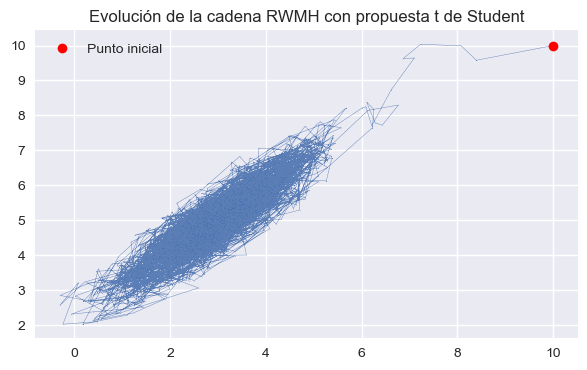
\includegraphics[width=0.7\textwidth]{tarea7/trajrwt.png}
        \end{center}

        Como vemos, en este caso también se cumple que la cadena entra en el conjunto de concentración
        de masa de la objetivo de manera relativamente rápida, y permanece ahí la mayor parte de la
        trayectoria. Para encontrar el \textit{burn-in} también graficamos únicamente la log-densidad
        de los primeros 1,000 puntos,

        \begin{center}
            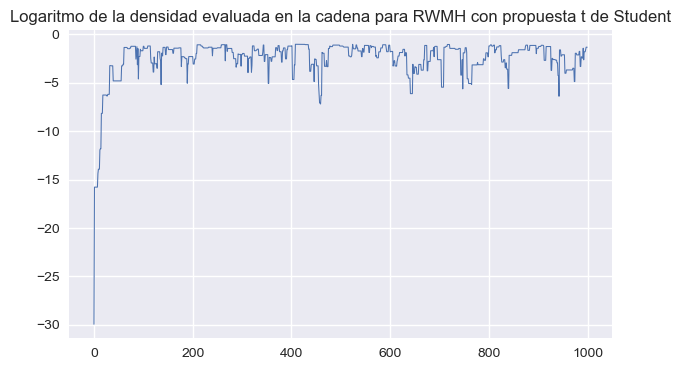
\includegraphics[width=0.7\textwidth]{tarea7/logdensrwt.png}
        \end{center}

        Nuevamente, podemos considerar que la cadena ha llegado a la zona de concentración de masa de la 
        objetivo en 100 pasos, o incluso menos. Al descartar las primeras 100 iteraciones de
        la cadena obtenemos los siguientes histogramas para las coordenadas de la distribución
        objetivo,

        \begin{center}
            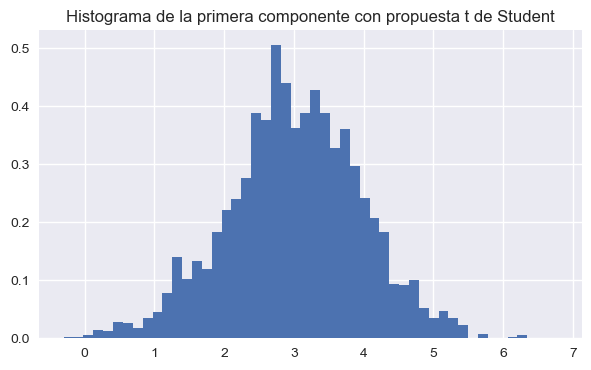
\includegraphics[width=0.7\textwidth]{tarea7/histrwt1.png}
            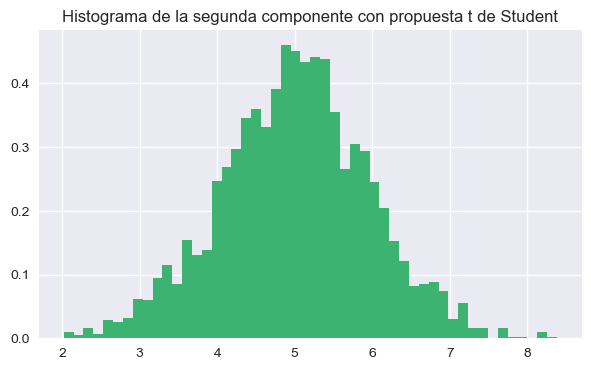
\includegraphics[width=0.7\textwidth]{tarea7/histrwt2.png}
        \end{center}

        Ambos histogramas son muy parecidos a los que se tenían en el caso en que la propuesta era 
        una normal multivariada, lo cual se justifica si consideramos que la distribución $t$ de Student
        multivariada es una aproximación a la distribución normal.
    \end{proof}



\textbf{Para todos los incisos del ejercicio anterior:}


\begin{itemize}
    \item Establece cual es tu distribución inicial.
    \item Grafica la evolución de la cadena.
    \item Indica cuál es el Burn-in.
    \item Comenta qué tan eficiente es la cadena.
    \item Implementa el algoritmo MH considerando una propuesta diferente.
\end{itemize}

Como conclusión, en todos los ejercicios anteriores notamos que existen decisiones 
sencillas en apariencia que pueden hacer una gran diferencia en el desempeño de un 
algoritmo de Metropolis-Hastings, por lo que el uso de esta técnica no se basa únicamente
en el conocimiento de la teoría, sino en la práctica necesaria para saber cuáles 
parámetros o distribuciones podrían resultar mejor en cada caso.

\end{enumerate}





 \end{document}